\documentclass[aspectratio=169]{beamer}

% ============================================================
% TEMA / ESTILO
% ============================================================
\usetheme{Madrid}
\usecolortheme{default}
\setbeamertemplate{navigation symbols}{}

\definecolor{myblue}{RGB}{0,183,235}
\definecolor{myred}{RGB}{160,30,30}
\definecolor{darkgray}{RGB}{70,70,70}

\setbeamercolor{title}{fg=myblue}
\setbeamercolor{frametitle}{fg=myblue}
\setbeamercolor{block title}{fg=myblue}
\setbeamercolor{alertblock title}{fg=myred}

% ============================================================
% PACOTES
% ============================================================
\usepackage[T1]{fontenc}
\usepackage[utf8]{inputenc}
\usepackage[brazil]{babel}
\usepackage{amsmath,amssymb,bm,mathtools}
\usepackage{physics}
\usepackage{tikz}
\usepackage{booktabs}
\usepackage{array}
\usepackage{multicol}
\usepackage{ragged2e}

\renewcommand{\arraystretch}{1.15}

% ============================================================
% COMANDOS
% ============================================================
\newcommand{\blue}[1]{\textcolor{myblue}{#1}}
\newcommand{\red}[1]{\textcolor{myred}{#1}}

\newcommand{\notas}[1]{%
\begin{tikzpicture}[remember picture,overlay]
\node[anchor=south west,
      xshift=3mm,
      yshift=3mm,
      draw,
      rectangle,
      rounded corners=2pt,
      fill=white,
      font=\tiny,
      inner sep=2pt]
at (current page.south west)
{Notas: #1};
\end{tikzpicture}
}

% ============================================================
% DADOS
% ============================================================
\title[FEX1]{Física Experimental 1}
\subtitle{Aula --- Gráficos em Física Experimental}
\author{Prof. Dr. Rafael C. R. de Lima}
\institute{UDESC --- CCT}
\date{\today}

\begin{document}

% ============================================================
\begin{frame}
\titlepage
\end{frame}

% ============================================================
\begin{frame}{Objetivos da Aula}
\begin{itemize}
\item Entender por que gráficos são fundamentais em Física Experimental.
\item Revisar o sistema de coordenadas cartesianas.
\item Aprender regras práticas para construir gráficos em papel milimetrado.
\item Discutir escolha de eixos, escalas, marcação de pontos e traçado da curva.
\item Aplicar o procedimento a um exemplo experimental com volume e temperatura.
\end{itemize}
\end{frame}

% ============================================================
\begin{frame}{Introdução}
\begin{itemize}
\item Entre os vários recursos de análise científica, os \textbf{gráficos} ocupam lugar de destaque.
\item Em vez de olhar apenas uma tabela de dados, o gráfico permite enxergar o
\textbf{comportamento geral} das grandezas físicas envolvidas.
\item Um gráfico bem construído resume visualmente muitas informações de uma medida.
\end{itemize}
\end{frame}

% ============================================================
\begin{frame}{Gráficos no Cotidiano}
Informações transmitidas por gráficos aparecem em muitas situações:

\begin{itemize}
\item evolução do salário mínimo;
\item mortalidade infantil;
\item número de furtos;
\item acidentes de trânsito;
\item ocupação de disco rígido;
\item funcionamento do coração e de outros órgãos.
\end{itemize}

\begin{block}{Ideia central}
Aprender a ``ler'' e construir gráficos é essencial para compreender dados.
\end{block}
\end{frame}

% ============================================================
\begin{frame}{Por que Gráficos são Importantes?}
\begin{itemize}
\item Um gráfico ajuda a \textbf{interpretar relações} entre grandezas físicas.
\item Permite visualizar como uma variável muda em relação a outra.
\item Mostra tendências, regularidades, comportamentos crescentes, decrescentes ou não lineares.
\item É uma linguagem visual extremamente poderosa em ciência e tecnologia.
\end{itemize}
\end{frame}

% ============================================================
\begin{frame}{Duas Grandezas Físicas}
Neste curso trabalharemos com gráficos envolvendo duas grandezas físicas:

\begin{itemize}
\item uma \textbf{variável independente};
\item uma \textbf{variável dependente}.
\end{itemize}

\bigskip

\begin{block}{Exemplo}
A velocidade pode depender do tempo: a grandeza independente é o tempo, e a dependente é a velocidade.
\end{block}
\end{frame}

% ============================================================
\begin{frame}{Mensagem do Texto}
\begin{alertblock}{Ponto importante}
Nas disciplinas de Física Experimental é indispensável o conhecimento e o domínio da construção e interpretação de gráficos.
\end{alertblock}

\begin{itemize}
\item Trabalharemos apenas com gráficos em papel milimetrado.
\item Mais adiante surgirão linearizações e outros tipos de papel.
\end{itemize}
\end{frame}

% ============================================================
\begin{frame}{Sistema de Coordenadas Cartesianas}
Considere uma grandeza dependente \(u\) que varia em função de uma grandeza independente \(z\):

\begin{equation}
u = f(z)
\end{equation}

Se a função é conhecida, ela pode ser representada em um sistema de coordenadas cartesianas.
\end{frame}

% ============================================================
\begin{frame}{Os Eixos Cartesianos}
O sistema de coordenadas cartesianas é composto por duas retas perpendiculares:

\begin{itemize}
\item eixo \(x\): eixo das abscissas;
\item eixo \(y\): eixo das ordenadas.
\end{itemize}

Na linguagem do texto:

\begin{itemize}
\item no eixo horizontal representamos a variável independente;
\item no eixo vertical representamos a variável dependente.
\end{itemize}
\end{frame}

% ============================================================
\begin{frame}{Pontos no Plano}
Cada par ordenado \((x_i,y_i)\) representa um ponto do gráfico.

No contexto do texto:

\begin{equation}
(x_i,y_i) = (z_i,u_i)
\end{equation}

Assim, o conjunto dos pontos experimentais representa visualmente a dependência de \(u\) em relação a \(z\).
\end{frame}

% ============================================================
\begin{frame}{Sinais e Quadrantes}
\begin{itemize}
\item Os eixos podem conter valores positivos ou negativos.
\item Isso depende do fenômeno estudado e da convenção adotada.
\item Em muitos problemas experimentais introdutórios trabalha-se apenas no quadrante em que as variáveis assumem valores positivos.
\end{itemize}
\end{frame}

% ============================================================
\begin{frame}{Figura III.1}
\begin{center}
\begin{figure}
    \centering
    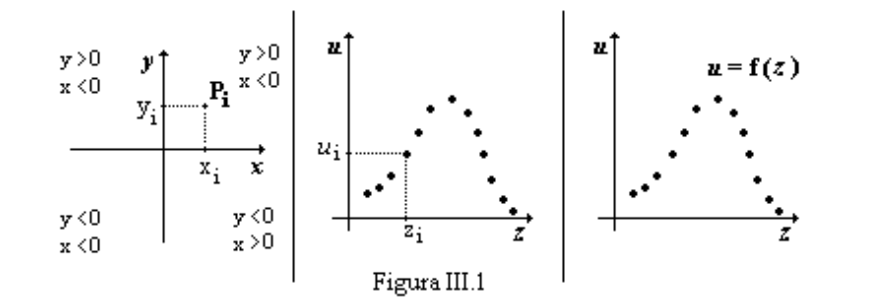
\includegraphics[width=0.7\linewidth]{III-1.png}
    \caption{Sistema Cartesiano e representação dos pontos experimentais}
    \label{fig:enter-label}
\end{figure}\end{center}
\end{frame}

% ============================================================
\begin{frame}{Construção de Gráficos em Papel Milimetrado}
A observação de um fenômeno físico geralmente começa com um \textbf{tabelamento de valores medidos}.

\bigskip

A partir da tabela, construímos o gráfico em papel milimetrado obedecendo a um conjunto de regras práticas.
\end{frame}

% ============================================================
\begin{frame}{Exemplo 15}
Em um experimento de dilatação volumétrica, mediu-se o volume \(V\) de uma esfera para várias temperaturas \(T\).

\bigskip

Os valores obtidos foram organizados em uma tabela com pares \((T_i,V_i)\).
\end{frame}

% ============================================================
\begin{frame}{Tabela de Dados do Exemplo 15}
\small
\begin{center}
\begin{tabular}{|c|c|c|c|c|c|c|c|c|c|}
\hline
\(V\,(10^{-9}\,\mathrm{m}^3)\) & 64,1 & 80,7 & 97,8 & 114,9 & 138,0 & 162,5 & 195,0 & 223,3 & 260,0 \\
\hline
\(T\,(^{\circ}\mathrm{C})\) & 60,00 & 65,00 & 70,00 & 75,00 & 80,00 & 85,00 & 90,00 & 95,00 & 100,00 \\
\hline
\(i\) & 1 & 2 & 3 & 4 & 5 & 6 & 7 & 8 & 9 \\
\hline
\end{tabular}
\end{center}
\end{frame}

% ============================================================
\begin{frame}{Leitura Física da Tabela}
Para cada par \((T_i,V_i)\):

\begin{itemize}
\item \(T_i\) é a temperatura medida;
\item \(V_i\) é o volume correspondente;
\item \(i\) apenas indica a ordem da medição.
\end{itemize}

\bigskip

Pela própria tabela já percebemos que, ao aumentar a temperatura, o volume também aumenta.
\end{frame}

% ============================================================
\begin{frame}{Qual Gráfico Devemos Fazer?}
Como o volume depende da temperatura, o gráfico correto é:

\begin{equation}
V \text{ versus } T
\end{equation}

ou seja:

\begin{itemize}
\item eixo horizontal: \(T\);
\item eixo vertical: \(V\).
\end{itemize}
\end{frame}

% ============================================================
\begin{frame}{Passo 1: Seleção do Papel}
No exemplo do texto, usaremos \textbf{papel milimetrado}.

\begin{itemize}
\item Em princípio, qualquer função de uma variável pode ser traçada nesse tipo de papel.
\item Mais adiante, outros tipos de papel serão estudados.
\end{itemize}
\end{frame}

% ============================================================
\begin{frame}{Passo 2: Definição dos Eixos}
\begin{itemize}
\item No eixo das abscissas (horizontal), registramos a \textbf{variável independente}.
\item No eixo das ordenadas (vertical), registramos a \textbf{variável dependente}.
\end{itemize}

\begin{block}{Regra prática}
Registramos a causa no eixo horizontal e o efeito no eixo vertical.
\end{block}
\end{frame}

% ============================================================
\begin{frame}{Exemplo Conceitual}
Se um experimentador mede a distância \(d\) percorrida por um corpo em função do tempo \(t\), o correto é:

\begin{equation}
d \text{ versus } t
\end{equation}

e não:

\begin{equation}
t \text{ versus } d
\end{equation}

\begin{alertblock}{Motivo}
A distância varia de acordo com o tempo, e não o contrário.
\end{alertblock}
\end{frame}

% ============================================================
\begin{frame}{Figura III.2}
\begin{center}
\begin{figure}
    \centering
    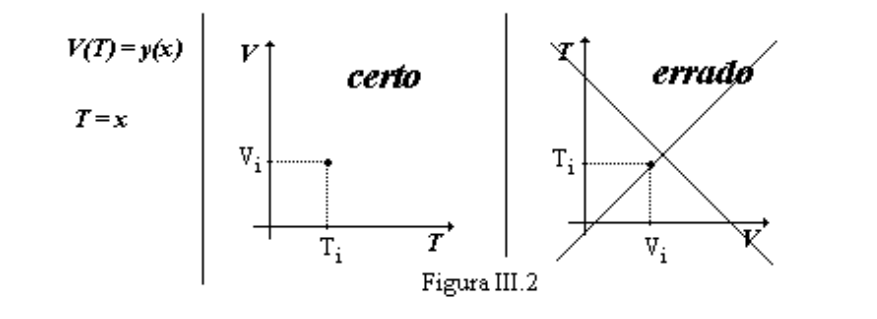
\includegraphics[width=0.7\linewidth]{III-2.png}
    \caption{Exemplo de escolha correta e incorreta dos eixos.}
    \label{fig:enter-label}
\end{figure}\end{center}
\end{frame}

% ============================================================
\begin{frame}{Passo 3: Registros dos Eixos}
Ao escrever os nomes das grandezas nos eixos:

\begin{itemize}
\item a variável independente deve aparecer junto ao eixo horizontal;
\item a variável dependente deve aparecer junto ao eixo vertical;
\item as unidades devem ser escritas entre parênteses.
\end{itemize}
\end{frame}

% ============================================================
\begin{frame}{Unidades nos Eixos}
A unidade física pode conter potência de 10, positiva ou negativa.

\bigskip

No exemplo:

\begin{equation}
V\,(10^{-9}\,\mathrm{m}^3)
\qquad \text{e} \qquad
T\,(^{\circ}\mathrm{C})
\end{equation}

\begin{block}{Importante}
A unidade deve ser registrada diretamente no gráfico.
\end{block}
\end{frame}

% ============================================================
\begin{frame}{Figura III.3}
\begin{center}
\begin{figure}
    \centering
    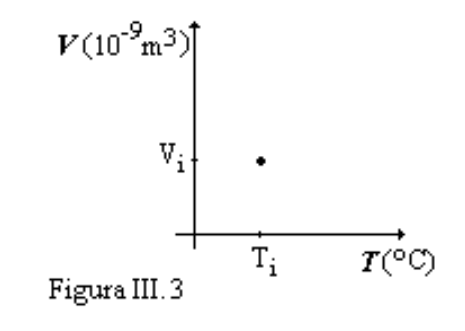
\includegraphics[width=0.6\linewidth]{III-3.png}
    \caption{Exemplo de registro correto das unidades nos eixos.}
    \label{fig:enter-label}
\end{figure}
\end{center}
\end{frame}

% ============================================================
\begin{frame}{Passo 4: Escalas e Posição do Papel}
A folha milimetrada usual tem aproximadamente:

\begin{itemize}
\item \(280\) mm no eixo vertical;
\item \(180\) mm no eixo horizontal.
\end{itemize}

Ela pode ser usada em duas posições:

\begin{itemize}
\item \textbf{retrato};
\item \textbf{paisagem}.
\end{itemize}
\end{frame}

% ============================================================
\begin{frame}{Critério Geral para Escalas}
\begin{itemize}
\item Devemos escolher uma escala que facilite a leitura dos pontos.
\item ``Ocupar bem a folha'' não significa necessariamente preencher toda a área disponível.
\item O essencial é usar uma \textbf{escala limpa, simples e fácil de ler}.
\end{itemize}

\begin{alertblock}{Evite}
Escalas que obriguem muitos cálculos mentais para localizar pontos.
\end{alertblock}
\end{frame}

% ============================================================
\begin{frame}{Variável Dependente: Volume}
No exemplo:

\begin{itemize}
\item valor mínimo aproximado: \(64{,}1\);
\item valor máximo: \(260{,}0\).
\end{itemize}

Momentaneamente ignoramos a unidade para facilitar a escolha da escala.
\end{frame}

% ============================================================
\begin{frame}{Volume no Papel em Retrato}
Se o papel estiver em posição \textbf{retrato}, o eixo vertical terá \(280\) mm.

\bigskip

Começando do zero:

\begin{equation}
260{,}0 \text{ unidades de volume}
\end{equation}

A escala direta mais simples é:

\begin{equation}
1{,}0 \text{ unidade de volume} : 1 \text{ mm do papel}
\end{equation}

Isso coloca o maior valor em \(260\) mm.
\end{frame}

% ============================================================
\begin{frame}{Volume em Retrato sem Começar do Zero}
Se começarmos, por exemplo, em \(60{,}0\), o intervalo útil é:

\begin{equation}
260{,}0 - 60{,}0 = 200{,}0
\end{equation}

Nesse caso, uma escala como \(1{,}0\) unidade por \(2\) mm ainda funciona bem, mas não é tão direta quanto a escolha anterior.
\end{frame}

% ============================================================
\begin{frame}{Conclusão para o Volume em Retrato}
\begin{block}{Escolha conveniente}
Na posição \textbf{retrato}, para o eixo vertical do volume, a melhor escolha é:

\begin{equation}
1{,}0 \text{ unidade de volume} : 1 \text{ mm do papel}
\end{equation}

começando do zero.
\end{block}
\end{frame}

% ============================================================
\begin{frame}{Volume no Papel em Paisagem}
Na posição \textbf{paisagem}, o eixo vertical passa a ter \(180\) mm.

\bigskip

Começando do zero, o intervalo de \(260{,}0\) unidades não cabe com a escala
\(1{,}0\) unidade por \(1\) mm.

\bigskip

Uma opção prática passa a ser:

\begin{equation}
2{,}0 \text{ unidades de volume} : 1 \text{ mm do papel}
\end{equation}
\end{frame}

% ============================================================
\begin{frame}{Conclusão para o Volume}
Comparando as duas orientações:

\begin{itemize}
\item em \textbf{retrato}, a escala para o volume fica mais direta;
\item em \textbf{paisagem}, o gráfico também pode ser feito, mas a escala fica menos natural.
\end{itemize}
\end{frame}

% ============================================================
\begin{frame}{Independência das Escalas}
\begin{alertblock}{Regra fundamental}
A escala usada em um eixo é totalmente independente da escala usada no outro.
\end{alertblock}

Isso significa que podemos escolher uma escala para o volume e outra completamente diferente para a temperatura.
\end{frame}

% ============================================================
\begin{frame}{Variável Independente: Temperatura}
Para a temperatura:

\begin{itemize}
\item valor mínimo: \(60{,}00\);
\item valor máximo: \(100{,}00\).
\end{itemize}

Logo, o intervalo relevante é muito menor do que o do volume.
\end{frame}

% ============================================================
\begin{frame}{Temperatura em Paisagem}
Se o papel estiver em \textbf{paisagem}, o eixo horizontal terá \(280\) mm.

\bigskip

Começando do zero, o intervalo de \(100\) unidades é pequeno para esse comprimento.

\bigskip

Uma escolha mais eficiente pode ser:

\begin{equation}
1{,}0 \text{ unidade de temperatura} : 2 \text{ mm do papel}
\end{equation}

ou, sem começar do zero, outra escala ainda mais espaçada.
\end{frame}

% ============================================================
\begin{frame}{Temperatura em Retrato}
Na posição \textbf{retrato}, o eixo horizontal terá \(180\) mm.

\bigskip

Começando em \(60{,}0\), o intervalo útil é:

\begin{equation}
100{,}0 - 60{,}0 = 40{,}0
\end{equation}

Uma escolha muito boa é:

\begin{equation}
1{,}0 \text{ unidade de temperatura} : 4 \text{ mm do papel}
\end{equation}
\end{frame}

% ============================================================
\begin{frame}{Melhor Combinação de Escalas}
Da análise feita no texto, a melhor ocupação da folha é:

\begin{itemize}
\item \textbf{posição do papel: retrato}
\item eixo vertical (volume): \(1{,}0\) unidade de volume para \(1\) mm do papel
\item eixo horizontal (temperatura): \(1{,}0\) unidade de temperatura para \(4\) mm do papel
\end{itemize}

Além disso, no eixo horizontal, o primeiro valor adotado será \(60{,}0\).
\end{frame}

% ============================================================
\begin{frame}{Conclusão das Escalas}
\begin{block}{Escolha final}
\begin{itemize}
\item Papel na posição \textbf{retrato}
\item Eixo vertical: volume \(V\)
\item Eixo horizontal: temperatura \(T\)
\item Escala do volume: \(1{,}0\) unidade por \(1\) mm
\item Escala da temperatura: \(1{,}0\) unidade por \(4\) mm
\end{itemize}
\end{block}
\end{frame}

% ============================================================
\begin{frame}{Passo 5: Indicação de Valores nos Eixos}
Os valores de referência ao longo dos eixos devem:

\begin{itemize}
\item ser compatíveis com a escala escolhida;
\item ser simples e legíveis;
\item preferencialmente usar múltiplos de 2, 5, 10, 20, 50, 100 etc.
\end{itemize}

\begin{alertblock}{Evite}
Múltiplos ou submúltiplos pouco naturais, como 3, 7, 9, 11, 13, 15 etc.
\end{alertblock}
\end{frame}

% ============================================================
\begin{frame}{Algarismos Significativos nos Eixos}
\begin{itemize}
\item Os valores marcados nos eixos devem respeitar a quantidade de algarismos significativos das medidas.
\item No caso do volume, por exemplo, podem aparecer marcações como:
\[
50{,}0,\quad 100{,}0,\quad 150{,}0,\quad \dots
\]
\end{itemize}
\end{frame}

% ============================================================
\begin{frame}{Passo 6: Marcação dos Pontos Experimentais}
\begin{itemize}
\item Os pontos devem ser marcados com clareza.
\item O símbolo escolhido deve permitir localizar o ponto sem ambiguidade.
\item Depois de marcar o ponto, não se deve acrescentar linhas auxiliares até os eixos.
\end{itemize}

\begin{block}{Regra prática}
Identifique apenas os pontos experimentais.
\end{block}
\end{frame}

% ============================================================
\begin{frame}{Figura III.4}
\begin{center}
\Large \textbf{[Inserir aqui a Figura III.4]}\\[1ex]
\normalsize Exemplos de símbolos para marcação dos pontos experimentais.
\end{center}
\end{frame}

% ============================================================
\begin{frame}{Passo 7: Traçado da Curva}
\begin{itemize}
\item O traçado da curva deve ser \textbf{suave e contínuo}.
\item A curva deve se ajustar o melhor possível ao conjunto de pontos experimentais.
\item Não se deve unir os pontos por segmentos de reta, pois isso sugeriria descontinuidades artificiais.
\end{itemize}
\end{frame}

% ============================================================
\begin{frame}{Sobre o Primeiro Ponto}
O texto chama atenção para um detalhe prático:

\begin{itemize}
\item o valor inicial da temperatura no eixo horizontal pode ser ligeiramente deslocado para a direita;
\item isso facilita a visualização dos pontos;
\item evita que o primeiro ponto fique ``colado'' ao eixo vertical.
\end{itemize}
\end{frame}

% ============================================================
\begin{frame}{Gráfico Final do Exemplo}
\begin{center}
\begin{figure}
    \centering
    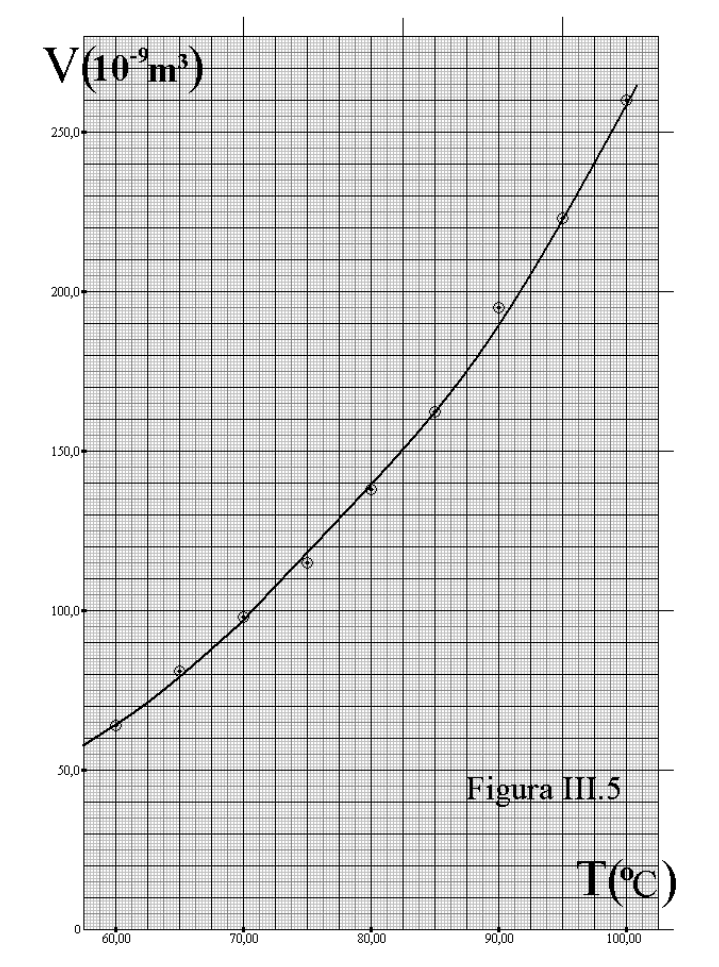
\includegraphics[width=0.3\linewidth]{III-5.png}
    \caption{Gráfico \(V\) versus \(T\) construído com as escalas escolhidas.}
    \label{fig:enter-label}
\end{figure}
\end{center}
\end{frame}

% ============================================================
\begin{frame}{Resumo do Procedimento}
Para construir um gráfico em papel milimetrado:

\begin{enumerate}
\item selecionar o papel;
\item definir os eixos;
\item registrar nomes e unidades;
\item escolher a posição do papel e as escalas;
\item indicar valores de referência;
\item marcar os pontos experimentais;
\item traçar a curva suavemente.
\end{enumerate}
\end{frame}

% ============================================================
\begin{frame}{Erros Comuns}
\begin{itemize}
\item inverter variável dependente e independente;
\item esquecer as unidades;
\item usar escalas difíceis de ler;
\item não respeitar algarismos significativos;
\item marcar pontos com ambiguidade;
\item ligar os pontos por segmentos de reta sem justificativa física.
\end{itemize}
\end{frame}


\begin{frame}{Gráfico Linear em Papel Milimetrado}
Nesta seção veremos como extrair informações físicas de um gráfico quando a curva traçada é uma reta.

\bigskip

Exemplo: movimento de um bloco deslizando em um plano inclinado.

\bigskip

A partir de medições experimentais de velocidade e tempo, podemos construir um gráfico e determinar parâmetros físicos do movimento.
\end{frame}


\begin{frame}{Dados Experimentais}
Foram obtidas as seguintes medições:

\begin{center}
\begin{tabular}{c|ccccccc}
$v\,(10^{-3}\,m/s)$ & 105 & 150 & 240 & 290 & 340 & 430 & 500\\
$t\,(10^{-2}\,s)$ & 1.00 & 2.50 & 6.00 & 8.00 & 10.00 & 13.50 & 16.00
\end{tabular}
\end{center}

Cada par $(t_i,v_i)$ será representado por um ponto no gráfico $v$ versus $t$.
\end{frame}


\begin{frame}{Gráfico Experimental}
\begin{center}
\begin{figure}
    \centering
    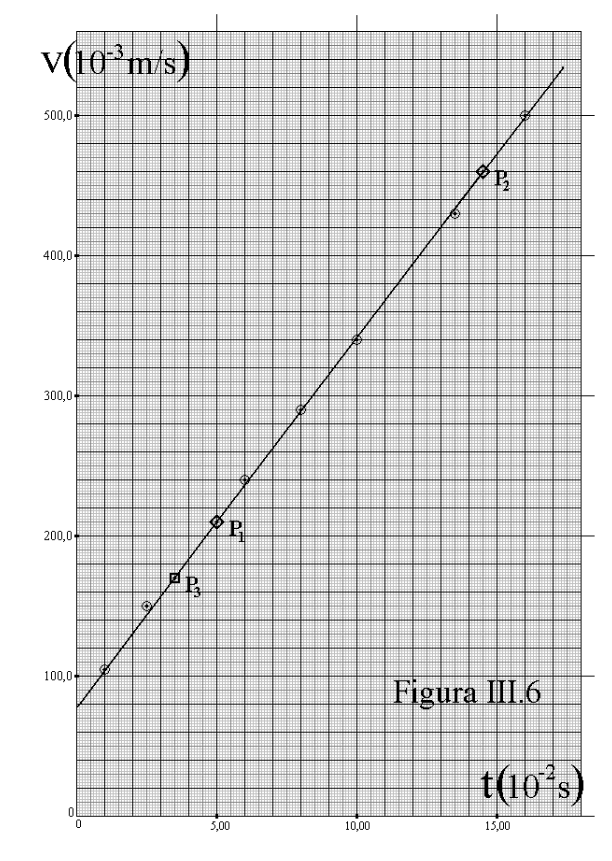
\includegraphics[width=0.25\linewidth]{III-6.png}
    \caption{Observamos que os pontos experimentais se alinham aproximadamente em uma reta.}
    \label{fig:enter-label}
\end{figure}\end{center}


\end{frame}


\begin{frame}{Equação da Reta}
Da geometria analítica:

\begin{equation}
y(x) = ax + b
\end{equation}

onde

\begin{itemize}
\item $a$ = coeficiente angular
\item $b$ = coeficiente linear
\end{itemize}

A partir do gráfico podemos determinar esses coeficientes.
\end{frame}


\begin{frame}{Coeficiente Angular}
O coeficiente angular é dado por

\begin{equation}
a = \frac{\Delta y}{\Delta x}
\end{equation}

ou

\begin{equation}
a = \frac{y_2-y_1}{x_2-x_1}
\end{equation}

onde $(x_1,y_1)$ e $(x_2,y_2)$ são dois pontos da reta.
\end{frame}


\begin{frame}{Escolha dos Pontos}
Importante:

\begin{block}{Regra}
Para calcular coeficientes da reta, não devemos usar pontos experimentais.
\end{block}

Devemos escolher pontos diretamente sobre a reta ajustada.
\end{frame}


\begin{frame}{Pontos Utilizados}
No gráfico foram escolhidos:

\[
P_1=(5.00\times10^{-2}s,\;210\times10^{-3}m/s)
\]

\[
P_2=(14.50\times10^{-2}s,\;460\times10^{-3}m/s)
\]
\end{frame}


\begin{frame}{Cálculo do Coeficiente Angular}

\[
a=\frac{v_2-v_1}{t_2-t_1}
\]

\[
a=\frac{(460-210)\times10^{-3}}{(14.50-5.00)\times10^{-2}}
\]

\[
a=2.63\,m/s^2
\]

\bigskip

O coeficiente angular corresponde à aceleração do movimento.
\end{frame}


\begin{frame}{Coeficiente Linear}
Existem duas maneiras de determinar o coeficiente linear.

\begin{itemize}
\item usar um ponto da reta
\item usar a interseção com o eixo
\end{itemize}
\end{frame}


\begin{frame}{Método 1}
Escolhe-se um ponto não experimental:

\[
P_3=(3.50\times10^{-2}s,\;170\times10^{-3}m/s)
\]

Usamos

\[
b=y-ax
\]

\[
b=78\times10^{-3}m/s
\]
\end{frame}


\begin{frame}{Método 2}
Podemos prolongar a reta até cortar o eixo vertical.

O valor de $v$ quando $t=0$ é:

\[
b=79\times10^{-3}m/s
\]
\end{frame}


\begin{frame}{Interpretação Física}
O coeficiente linear corresponde à:

\begin{block}{Velocidade inicial}
$v_0$
\end{block}

Portanto

\[
v(t)=at+v_0
\]
\end{frame}


\begin{frame}{Equação do Movimento}

\[
v(t)= (2.63\,m/s^2)t + (79\times10^{-3}m/s)
\]

com $t$ em segundos.
\end{frame}


\begin{frame}{Introdução à Linearização}
Nem sempre os dados produzem uma reta.

Muitas vezes o gráfico é curvo.

Nesse caso utilizamos uma técnica chamada:

\begin{block}{Linearização}
Transformar um gráfico curvo em um gráfico linear.
\end{block}
\end{frame}


\begin{frame}{Exemplo de Movimento}
Considere medições da posição de um móvel:

\begin{center}
\begin{tabular}{c|cccccc}
$x(m)$ & 58 & 84 & 105 & 150 & 188 & 240\\
$t(s)$ & 5.25 & 7.00 & 8.00 & 10.00 & 11.50 & 13.00
\end{tabular}
\end{center}
\end{frame}


\begin{frame}{Gráfico Original}
\begin{center}
\begin{figure}
    \centering
    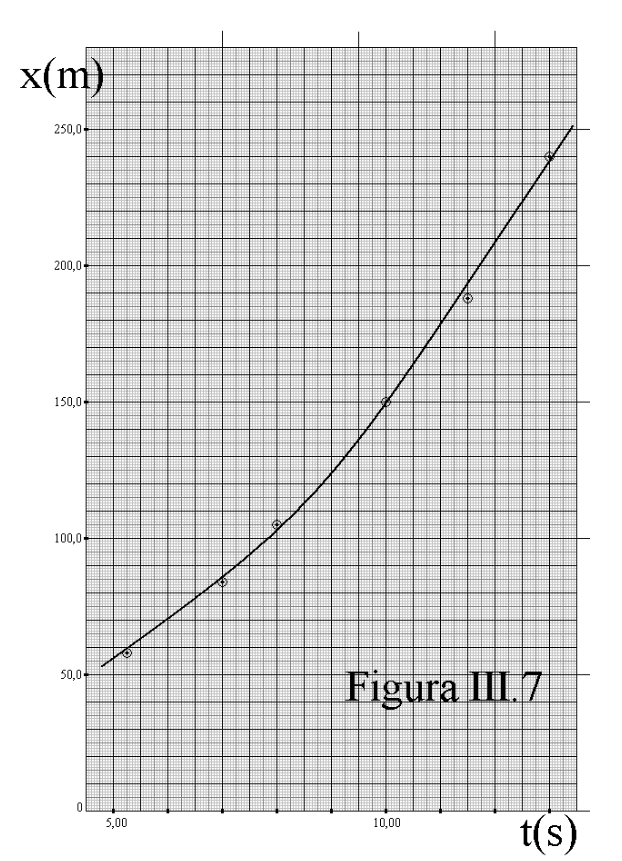
\includegraphics[width=0.27\linewidth]{III-7.png}
    \caption{A curva obtida não é uma reta.}
    \label{fig:enter-label}
\end{figure}\end{center}


\end{frame}


\begin{frame}{Equação do Movimento}
A equação pode ser escrita como

\[
x(t)=\epsilon t^2+\gamma
\]

onde $\epsilon$ e $\gamma$ são constantes.
\end{frame}


\begin{frame}{Ideia da Linearização}
Comparando com a equação da reta

\[
y=ax+b
\]

fazemos a mudança

\[
x \rightarrow t^2
\]

Assim o gráfico $x$ versus $t^2$ será uma reta.
\end{frame}


\begin{frame}{Nova Tabela}
Calculamos $t^2$:

\begin{center}
\begin{tabular}{c|cccccc}
$x(m)$ & 58 & 84 & 105 & 150 & 188 & 240\\
$t(s)$ & 5.25 & 7.00 & 8.00 & 10.00 & 11.50 & 13.00\\
$t^2(s^2)$ & 27.6 & 49.0 & 64.0 & 100.0 & 132.2 & 169.0
\end{tabular}
\end{center}
\end{frame}


\begin{frame}{Gráfico Linearizado}
\begin{center}
\begin{figure}
    \centering
    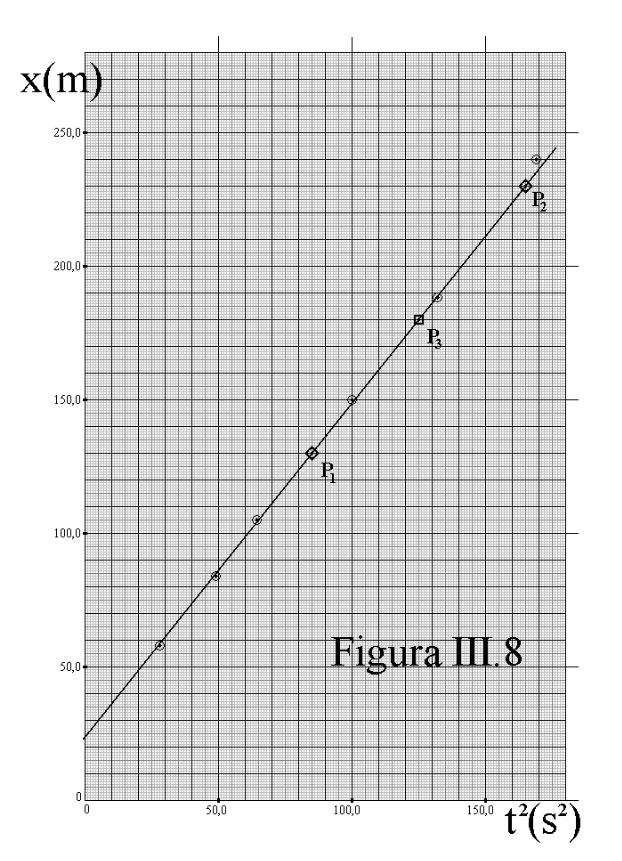
\includegraphics[width=0.27\linewidth]{III-8.png}
    \caption{Agora obtemos uma reta.}
    \label{fig:enter-label}
\end{figure}\end{center}


\end{frame}


\begin{frame}{Coeficiente Angular}
Escolhendo dois pontos da reta:

\[
\epsilon=1.25\,m/s^2
\]

Este coeficiente também corresponde a uma aceleração.
\end{frame}


\begin{frame}{Coeficiente Linear}

\[
\gamma = 23.8\,m
\]

ou aproximadamente

\[
\gamma \approx 24\,m
\]

Este valor corresponde à posição inicial do móvel.
\end{frame}


\begin{frame}{Resultado Final}
\[
x(t)=\epsilon t^2+\gamma
\]

\[
x(t)=(1.25\,m/s^2)t^2 + 24m
\]

Sabendo que no movimento uniformemente acelerado

\[
x(t)=x_0+v_0t+\frac12\alpha t^2
\]

obtemos

\[
\alpha = 2.50\,m/s^2
\]
\end{frame}

% ============================================================
\begin{frame}{Mensagem Final}
\begin{block}{Conclusão}
Um gráfico bem construído não é apenas um desenho bonito: ele é uma forma rigorosa de representar e interpretar dados experimentais.
\end{block}

\begin{itemize}
\item Clareza
\item Fidelidade aos dados
\item Escalas limpas
\item Leitura fácil
\end{itemize}
\end{frame}

% ============================================================
\begin{frame}{Exercícios Sugeridos}
\begin{itemize}
\item Reproduza o gráfico do Exemplo 15 em papel milimetrado.
\item Teste outra escolha de escalas e compare a legibilidade.
\item Escolha uma nova tabela de dados e determine:
\begin{itemize}
\item variável dependente;
\item variável independente;
\item posição do papel;
\item escalas adequadas.
\end{itemize}
\end{itemize}
\end{frame}

% ============================================================
\begin{frame}{Encerramento}
\begin{center}
\Large Bom estudo!
\end{center}
\end{frame}

\end{document}